%=======================================================================
\section{Array Component} \label{s:component-array}
%=======================================================================

Use chunked field storage \\
Field chunk size or range
The \code{Array} classes encapsulate Fortran-style arrays with
convenient operations and optional special features.  

Optional features include storing as a blocked array to improve cache
use, array padding to avoid cache thrashing on large power-of-two
arrays with low-associativity caches.  Arrays also may be parallelized
according to \code{Parallel} objects such as
\code{Parallel::Mpi} for MPI-parallel distributed arrays, or
\code{Parallel::Omp} for OpenMP-parallel threaded arrays (or both).

To manage the various optional features, Array classes use the
Decorator design pattern for dynamically adding special features at
run time:

 \centerline{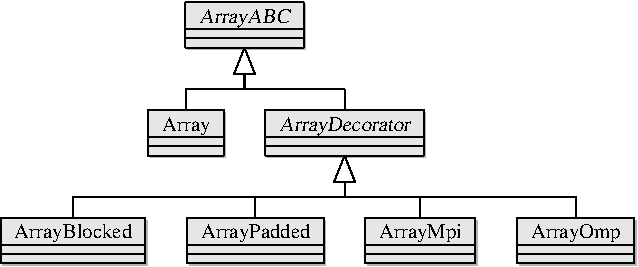
\includegraphics{uml/arrays.ps}}

\subsection{\code{Array}}

\centerline{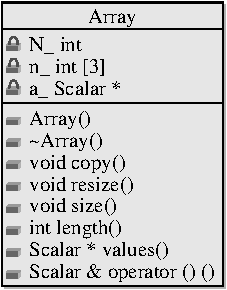
\includegraphics{uml/array.ps}}

\subsubsection{Array shape}

\subsubsection{Array blocking}

\subsubsection{Array padding}

\subsubsection{Array interleaving}


\subsection{Attributes}

\begin{tabbing}
xx\=xx\=xxxxxxxxxxxxxxxxxxxxxxxxxxxxxxxxxxx\= \kill
\> \todo \>  \textit{Length of array} \\
\>       \> \code{N\_: int }      \\ \\
\> \todo \>  \textit {Shape of array, right-padded with 1's} \\
\>       \> \code{n\_: int [3] }  \\ \\
\> \todo \>  \textit {Array values stored in column-major ordering}\\
\>       \> \code{a\_: Scalar * }
\end{tabbing}

\subsection{Operations}

\begin{tabbing}
xx\=xx\=xxxxxxxxxxxxxxxxxxxxxxxxxxxxxxxxxxx\= \kill
\> \todo \> \textit{Create a new uninitialized Array object} \\
\>       \> \code{Array()} \\ \\
\> \todo \> \textit{Create a new initialized Array object} \\
\>       \> \code{Array(int n0, int n1=1, int n2=1, int n3=1)} \\ \\
\> \todo \> \textit{Deallocate the array} \\
\>       \> \code{\~{\ }Array()}  \\ \\
\> \todo \> \textit{Copy an array into this one, deallocating any existing data} \\
\>       \> \code{void copy (const Array \&)}  \\ \\
\> \todo \> \textit{Resize the array, deallocating any existing data} \\
\>       \> \code{void resize (int n0, int n1=1, int n2=1, int n3=1)}   \\ \\
\> \todo \> \textit{Return the size of the array} \\
\>       \> \code{void size (int *n0, int *n1=0, int *n2=0, int *n3=0) const}  \\ \\
\> \todo \> \textit{Return the total length of the array} \\
\>       \> \code{int length () const}  \\ \\
\> \todo \> \textit{Return a pointer to the array values} \\
\>       \> \code{Scalar * values () const}  \\ \\
\> \todo \> \textit{Return the given array element} \\
\>       \> \code{Scalar \& operator () (int i0, int i1=0, int i2=0, int i3=0)}
\end{tabbing}


